\documentclass[12pt,a4paper,openright,twoside]{book}
\usepackage[utf8]{inputenc}
\usepackage{disi-thesis}
\usepackage{code-lstlistings}
\usepackage{notes}
\usepackage{shortcuts}
\usepackage{acronym}

\school{\unibo}
\programme{Corso di Laurea in Ingegneria e Scienze Informatiche}
\title{Monitoraggio Ed Automazione Della Distribuzione Di Software Complessi}
\author{Marco Sternini}
\date{\today}
\subject{Programmazione ad oggetti}
\supervisor{Dott. Danilo Pianini}
\cosupervisor{Dott.sa Martina Baiardi}
\session{III}
\academicyear{2022-2023}

% Definition of acronyms
\acrodef{vm}[VM]{Virtual Machine}
\acrodef{cicd}[CI/CD]{Continuous Integration Continuous Delivery}
\acrodef{cli}[CLI]{Command Line Interface}
\acrodef{jvm}[JVM]{Java Virtual Machine}
\acrodef{jre}[JRE]{Java Runtime Environment}
\acrodef{aur}[AUR]{Arch User Repository}

\mainlinespacing{1.241} % line spacing in mainmatter, comment to default (1)

\begin{document}

\frontmatter\frontispiece

\begin{abstract}	
Max 2000 characters, strict.
\end{abstract}

\begin{dedication} % this is optional
Optional. Max a few lines.
\end{dedication}

\begin{acknowledgements} % this is optional
Optional. Max 1 page.
\end{acknowledgements}

%----------------------------------------------------------------------------------------
\tableofcontents   
\listoffigures     % (optional) comment if empty
\lstlistoflistings % (optional) comment if empty
%----------------------------------------------------------------------------------------

\mainmatter

%----------------------------------------------------------------------------------------
\chapter{Introduzione}
\label{chap:introduction}
%----------------------------------------------------------------------------------------

Introduzione 

(Il problema, software oggigiorno, l'importanza della qualità del software e altre caratteristiche di ingegneria del software, come automatizzare migliora la qualità eliminando l'intervento umano)

\begin{figure}
	\centering
	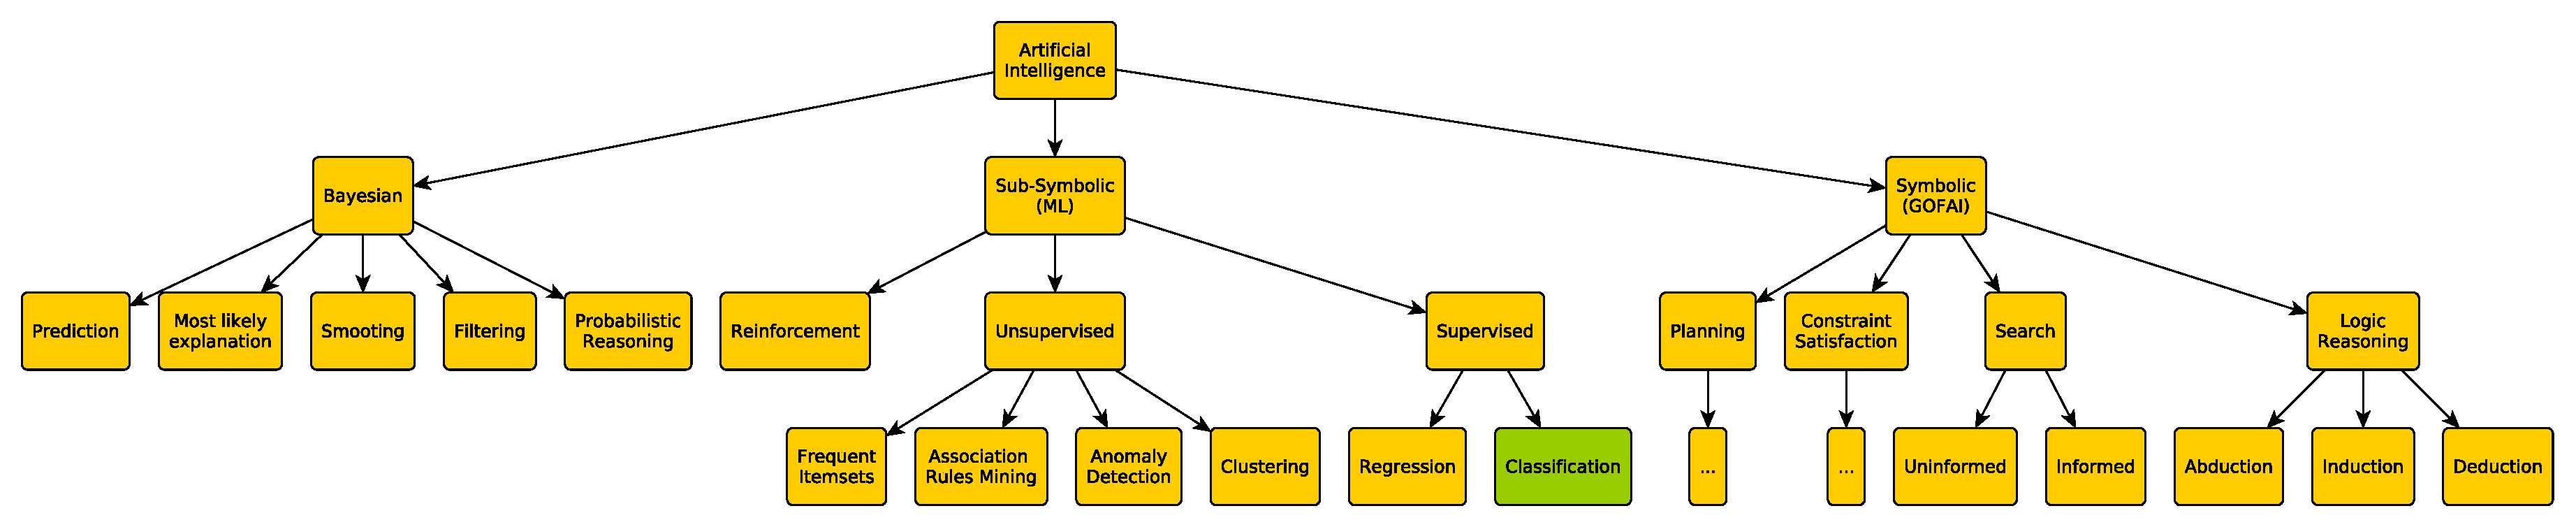
\includegraphics[width=.8\linewidth]{figures/random-image.pdf}
	\caption{Some random image}
	\label{fig:random-image}
\end{figure}

\section{Contesto}

(Un'introduzione teorica degli elementi sotto elencati, cosa servono, esempi di software che risolvono questo problema, evoluzione di questi negli ultimi anni )

\subsection{Build automation}
\subsection{Continuous integration}
\subsection{Continuous delivery}
\subsection{Alchemist}

(Cos'è alchemist, utilizzo, tecnologie utilizzate, architettura, progettazione)

\section{Obiettivi}

\paragraph{Struttura della tesi}

La struttura di questo paper

\chapter{Analisi}

Il progetto si pone tre principali obiettivi:
\begin{itemize}
	\item L'automazione della generazione di pacchetti di installazione multi-piattaforma con \ac{jre} integrato
	\item La pubblicazione automatica dei rilasci all'interno dell'\ac{aur}
	\item Lo sviluppo di una \ac{cli} per interagire con il simulatore
\end{itemize}

% JRE-Embed
Le applicazioni basate sulla \ac{jvm} necessitano di un \ac{jre}, ovvero un insieme di librerie e componenti che ne permettono l'esecuzione. L'utente potrebbe non aver alcun \ac{jre} installato sul proprio dispositivo oppure quello presente potrebbe essere obsoleto. Una soluzione consiste nel distribuire la propria applicazione assieme ad un \ac{jre} risultando in un maggiore controllo sull'ambiente di esecuzione e la semplificazione dell'installazione dell'applicativo, a discapito di un aumento delle dimensioni del software. La pacchettizzazione 

\section{Requisiti}

\subsection{Requisiti funzionali}
\begin{itemize}
	\item L'automazione della generazione di pacchetti di installazione multi-piattaforma con \ac{jre} integrato
	\item La pubblicazione automatica dei rilasci all'interno dell'\ac{aur}
	\item Lo sviluppo di una \ac{cli} per interagire con il simulatore
\end{itemize}

\subsection{Requisiti non funzionali}
\begin{itemize}
	\item L'automazione della generazione di pacchetti di installazione multi-piattaforma con \ac{jre} integrato
	\item La pubblicazione automatica dei rilasci all'interno dell'\ac{aur}
	\item Lo sviluppo di una \ac{cli} per interagire con il simulatore
\end{itemize}

\section{Strumenti}

\subsection{Gradle}

\subsection{Github actions}

\subsection{Arch User Repository}

\chapter{Design}

\section{Architettura e macrostruttura}
Interazione tra gradle e github actions, l’attuale struttura della pipeline di alchemist, le aggiunte che sono state fatte..

\section{Impacchettamento}
Discussione sulla scelta del software di packaging, il packaging di un progetto JVM, vantaggi / svantaggi

\subsection{GraalVM}

\subsection{JPackage}

\subsection{Valutazioni}

\section{Flusso di rilascio}
Il processo del rilascio di una release nuova di alchemist, dalle automazioni già presenti alle integrazioni di testing, impacchettamento e pubblicazione
\subsection{Rilascio}

\subsection{Pubblicazione}

\section{User experience}
Discussione design della terza parte

\subsection{CLI e GUI}

\subsection{Design CLI}

\chapter{Implementazione}

\begin{list}{possibili inserimenti}{spacing}
	\item Particolari design nell'interfaccia CLI
	\item Esempi
\end{list}

\chapter{Conclusioni}

\section{Sviluppi futuri}

%----------------------------------------------------------------------------------------
% BIBLIOGRAPHY
%----------------------------------------------------------------------------------------

\backmatter

\nocite{*} % comment this to only show the referenced entries from the .bib file

\bibliographystyle{alpha}
\bibliography{bibliography}

\end{document}